%%%%%%%%%%%%%%%%%%%%%%%%%%%%%%%%%%%%%%%%%
% Masters/Doctoral Thesis 
% LaTeX Template
% Version 3 (07/08/2021)
%
% modified by Kadek Ananta Satriadi (kadeksatriadi.com or ka.satriadi@gmail.com)
% 
%
%This template was downloaded from:
% http://www.LaTeXTemplates.com
%
% Version 2.x major modifications by:
% Vel (vel@latextemplates.com)
%
% This template is based on a template by:git
% Steve Gunn (http://users.ecs.soton.ac.uk/srg/softwaretools/document/templates/)
% Sunil Patel (http://www.sunilpatel.co.uk/thesis-template/)
%
% Template license:
% CC BY-NC-SA 3.0 (http://users.ecs.soton.ac.uk/srg/softwaretools/document/templates/)
%
%%%%%%%%%%%%%%%%%%%%%%%%%%%%%%%%%%%%%%%%%

%----------------------------------------------------------------------------------------
%	PACKAGES AND OTHER DOCUMENT CONFIGURATIONS
%----------------------------------------------------------------------------------------

\documentclass[
12pt, twoside, % The default document font size, options: 10pt, 11pt, 12pt
%oneside, % Two side (alternating margins) for binding by default, uncomment to switch to one side
english, % ngerman for German
onehalfspacing, % Single line spacing, alternatives: onehalfspacing or doublespacing
%draft, % Uncomment to enable draft mode (no pictures, no links, overfull hboxes indicated)
%nolistspacing, % If the document is onehalfspacing or doublespacing, uncomment this to set spacing in lists to single
liststotoc, % Uncomment to add the list of figures/tables/etc to the table of contents
%toctotoc, % Uncomment to add the main table of contents to the table of contents
parskip, % Uncomment to add space between paragraphs
%nohyperref, % Uncomment to not load the hyperref package
%headsepline, % Uncomment to get a line under the header
chapterinoneline, % Uncomment to place the chapter title next to the number on one line
%consistentlayout, % Uncomment to change the layout of the declaration, abstract and acknowledgements pages to match the default layout
]{MastersDoctoralThesis} % The class file specifying the document structure

% CUSTOMISATION added by Kadek
% Resources
% https://tex.stackexchange.com/questions/534406/problem-with-natbibapa-and-shortcite
% https://tex.stackexchange.com/questions/466819/use-round-brackets-instead-of-square-brackets-in-natbib-citations
%https://tex.stackexchange.com/questions/375413/how-to-make-last-names-of-authors-appear-first-in-my-bibliography
\usepackage[round]{natbib}
\usepackage{hyphenat} %hyphenation
\usepackage{graphicx}
\usepackage{grffile}
\usepackage{array }
\usepackage{rotating} %rotate table
\newcommand{\refsecname}[1]{\autoref{#1}. \nameref{#1}} % ref section with numbering and name
\newcommand{\refsecnamenosec}[1]{ \nameref{#1}} % ref section with numbering and name
\usepackage{pdfpages} %Include pdf
\usepackage{wrapfig} % Wrap figure
\usepackage[toc,page]{appendix} %appendicies
\usepackage{amssymb} % list symbol
\KOMAoptions{draft=false}% <- disables the draft mode for scrlayer-scrpage
\usepackage[utf8]{inputenc} % Required for inputting international characters
%\usepackage[T1]{fontenc} % Output font encoding for international characters
%\renewcommand*\familydefault{\sfdefault} %% Only if the base font of the document is to be sans serif
%\usepackage{mathpazo} % Use the Palatino font by default
\usepackage[sfdefault]{quattrocento}
\usepackage[T1]{fontenc}
%\usepackage[autostyle=true]{csquotes} % Required to generate language-dependent quotes in the bibliography
\usepackage{titlesec, blindtext, color}
\definecolor{gray75}{gray}{0.75}
\newcommand{\hsp}{\hspace{20pt}}

\titleformat{\chapter}[hang]{\color{NavyBlue}\fontfamily{phv}\Huge\raggedright}{\thechapter\hsp\textcolor{NavyBlue}{|}\hsp}{0pt}{\Huge}
\titleformat*{\section}{\color{NavyBlue}\fontfamily{phv}\Large\raggedright}
\titleformat*{\subsection}{\color{NavyBlue}\fontfamily{phv}\large\raggedright}


%GRAPHICS
\graphicspath{
{Chapters/Paper1/figures/}{Chapters/Paper1/},
{Chapters/Paper2/figures/}{Chapters/Paper2/},
{Chapters/Paper3/figures/}{Chapters/Paper3/}
}

% END CUSTOMISATION

%----------------------------------------------------------------------------------------
%	MARGIN SETTINGS
%----------------------------------------------------------------------------------------

\geometry{
	paper=a4paper, % Change to letterpaper for US letter
	inner=2.5cm, % Inner margin
	outer=3.8cm, % Outer margin
	bindingoffset=.5cm, % Binding offset
	top=1.5cm, % Top margin
	bottom=1.5cm, % Bottom margin
	%showframe, % Uncomment to show how the type block is set on the page
}

%----------------------------------------------------------------------------------------
%	THESIS INFORMATION
%----------------------------------------------------------------------------------------

\thesistitle{Your Awesome Thesis Title} % Your thesis title, this is used in the title and abstract, print it elsewhere with \ttitle
\supervisor{Your Awesome Supervisor} % Your supervisor's name, this is used in the title page, print it elsewhere with \supname
\examiner{} % Your examiner's name, this is not currently used anywhere in the template, print it elsewhere with \examname
\degree{Doctor of Philosophy} % Your degree name, this is used in the title page and abstract, print it elsewhere with \degreename
\author{Your Name} % Your name, this is used in the title page and abstract, print it elsewhere with \authorname
\addresses{} % Your address, this is not currently used anywhere in the template, print it elsewhere with \addressname

\subject{Your Subject} % Your subject area, this is not currently used anywhere in the template, print it elsewhere with \subjectname
\keywords{} % Keywords for your thesis, this is not currently used anywhere in the template, print it elsewhere with \keywordnames
\university{Your University} % Your university's name and URL, this is used in the title page and abstract, print it elsewhere with \univname
\department{Departement} % Your department's name and URL, this is used in the title page and abstract, print it elsewhere with \deptname
\group{Your Awesome Group} % Your research group's name and URL, this is used in the title page, print it elsewhere with \groupname
\faculty{Faculty} % Your faculty's name and URL, this is used in the title page and abstract, print it elsewhere with \facname

\AtBeginDocument{
\hypersetup{pdftitle=\ttitle} % Set the PDF's title to your title
\hypersetup{pdfauthor=\authorname} % Set the PDF's author to your name
\hypersetup{pdfkeywords=\keywordnames} % Set the PDF's keywords to your keywords
}

\begin{document}

\frontmatter % Use roman page numbering style (i, ii, iii, iv...) for the pre-content pages

\pagestyle{plain} % Default to the plain heading style until the thesis style is called for the body content

%----------------------------------------------------------------------------------------
%	TITLE PAGE
%----------------------------------------------------------------------------------------

\begin{titlepage}
	\begin{center}
		
		%{\scshape\LARGE \univname\par}\vspace{1.5cm} % University name
		%\textsc{\Large Doctoral Thesis}\\[0.5cm] % Thesis type
		
		\begin{figure}
			\centering
			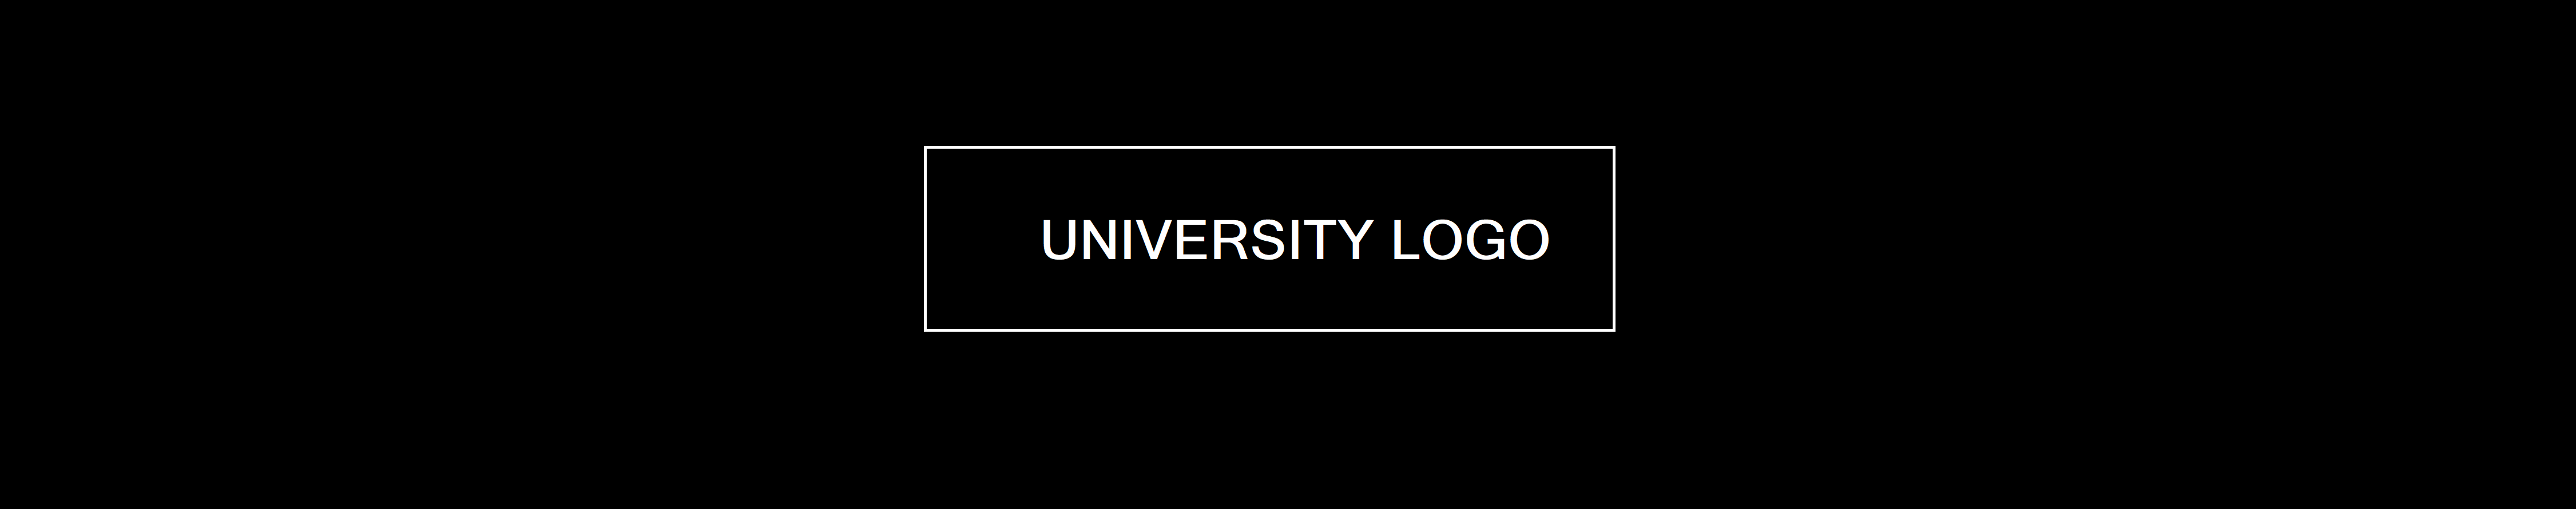
\includegraphics[width=\linewidth]{Figures/logo.png} %University Logo
		\end{figure}
		
	    \vspace{5cm}
		%\HRule \\[0.4cm] % Horizontal line
		{\fontfamily{phv} \Large \textbf{\ttitle}\par}% Thesis title
		%\HRule \\[1cm] % Horizontal line
		\vspace{1cm}
		{{\large \authorname}}
		
		{\small Your Degree}			\\[0.4cm]
		
		\vspace{1cm}

		\large A thesis submitted for the degree of Doctor of Philosophy at  % University requirement text

        \large Monash University in 2021 \\[0.5cm]
		%\\[0.4cm]
		\small
		\groupname\\
		\deptname\\
		\facname\\[2cm] % Research group name and department name
		
		\normalsize
	\begin{minipage}[t]{0.4\textwidth}
		\centering
		\emph{Main supervisor:} \\
		{\supname}		
		\vspace{0.25cm}

		\emph{Associate supervisors:} \\
		Associate supervisor1\\
		Associate supervisor2\\


	\end{minipage}
	
	\end{center}
\end{titlepage}

\newpage
%POST COVER
\vspace*{\fill}
\begin{small}

\textbf{\authorname} 

\textit{\ttitle}

A thesis submitted for the degree of Doctor of Philosophy, August 2021\\
Main supervisor: \supname\\
Associate supervisors:  \\
Examiners: 

\textbf{\univname}

Your Lab\\
\deptname\\
\facname\\
Address of your faculty.

\vspace{1cm}
\begin{footnotesize}
The style of this thesis is based on the Doctoral Thesis template from\\
\url{https://github.com/KadekSatriadi/phd-thesis-latex-template}.\\CC BY-NC-SA 3.0 license.


\end{footnotesize}

\end{small}

% COPYRIGHT NOTICE
\chapter*{Copyright Notice}

©\authorname (2021). 

\vspace{\baselineskip}

\noindent I certify that I have made all reasonable efforts to secure copyright permissions for third-party content included in this thesis and have not knowingly added copyright content to my work without the owner's permission.


% ABSTRACT
\chapter*{Abstract}
This thesis is awesome. Read me. 

% PUBLICATION
\chapter*{Publications During Enrolment}
\Large
Publications included in this thesis.
\normalsize

List of your publications presented in this thesis. 

\vspace{1cm}
\Large
Other publications not included in this thesis.
\normalsize

List of your publications that are not included in this thesis. 

% INCLUDING PUBLSIHED WORK
\chapter*{Thesis Including Published Works Declaration}
This is the declaration of authorship of publications included in this theis. While this could be found in the thesis by publication, you might not need this. 
Refer to your university's requirements. 

%\includepdf{contribution-statement.pdf} 




%	ACKNOWLEDGEMENTS
\chapter*{Acknowledgments}
I owe a debt of gratitude to my supervisors ... 

%----------------------------------------------------------------------------------------
%	LIST OF CONTENTS/FIGURES/TABLES PAGES
%----------------------------------------------------------------------------------------
\setcounter{secnumdepth}{2}
\setcounter{tocdepth}{1}

\tableofcontents % Prints the main table of contents

\listoffigures % Prints the list of figures

\listoftables % Prints the list of tables

%----------------------------------------------------------------------------------------
%	ABBREVIATIONS
%----------------------------------------------------------------------------------------

%\begin{abbreviations}{ll} % Include a list of abbreviations (a table of two columns)

%\textbf{LAH} & \textbf{L}ist \textbf{A}bbreviations \textbf{H}ere\\
%\textbf{WSF} & \textbf{W}hat (it) \textbf{S}tands \textbf{F}or\\

%\end{abbreviations}

%----------------------------------------------------------------------------------------
%	PHYSICAL CONSTANTS/OTHER DEFINITIONS
%----------------------------------------------------------------------------------------

%\begin{constants}{lr@{${}={}$}l} % The list of physical constants is a three column table

% The \SI{}{} command is provided by the siunitx package, see its documentation for instructions on how to use it

%Speed of Light & $c_{0}$ & \SI{2.99792458e8}{\meter\per\second} (exact)\\
%Constant Name & $Symbol$ & $Constant Value$ with units\\

%\end{constants}

%----------------------------------------------------------------------------------------
%	SYMBOLS
%----------------------------------------------------------------------------------------

%\begin{symbols}{lll} % Include a list of Symbols (a three column table)

%$a$ & distance & \si{\meter} \\
%$P$ & power & \si{\watt} (\si{\joule\per\second}) \\
%Symbol & Name & Unit \\

%\addlinespace % Gap to separate the Roman symbols from the Greek

%$\omega$ & angular frequency & \si{\radian} \\

%\end{symbols}

%----------------------------------------------------------------------------------------
%	DEDICATION
%----------------------------------------------------------------------------------------

%\dedicatory{For/Dedicated to/To my\ldots} 



\mainmatter % Begin numeric (1,2,3...) page numbering

\pagestyle{thesis} % Return the page headers back to the "thesis" style

% Include the chapters of the thesis as separate files from the Chapters folder
% Uncomment the lines as you write the chapters
%----------------------------------------------------------------------------------------
%	THESIS CONTENT - CHAPTERS
%----------------------------------------------------------------------------------------
\chapter{Introduction}
An awesome introduction.
\chapter{Background}
This is your awesome background chapter. 
\chapter{Paper 1 - Awesome Paper}
This is your first paper chapter. 

\newpage
This page demonstrates the footer style of this template. 

\newpage
The style of this thesis is ``twoside'', meaning the footer on the odd page and even page is formatted differently.

\newpage
This is an example of a figure, obtained from \citet{wiki1}. 

\begin{figure}[hb!]
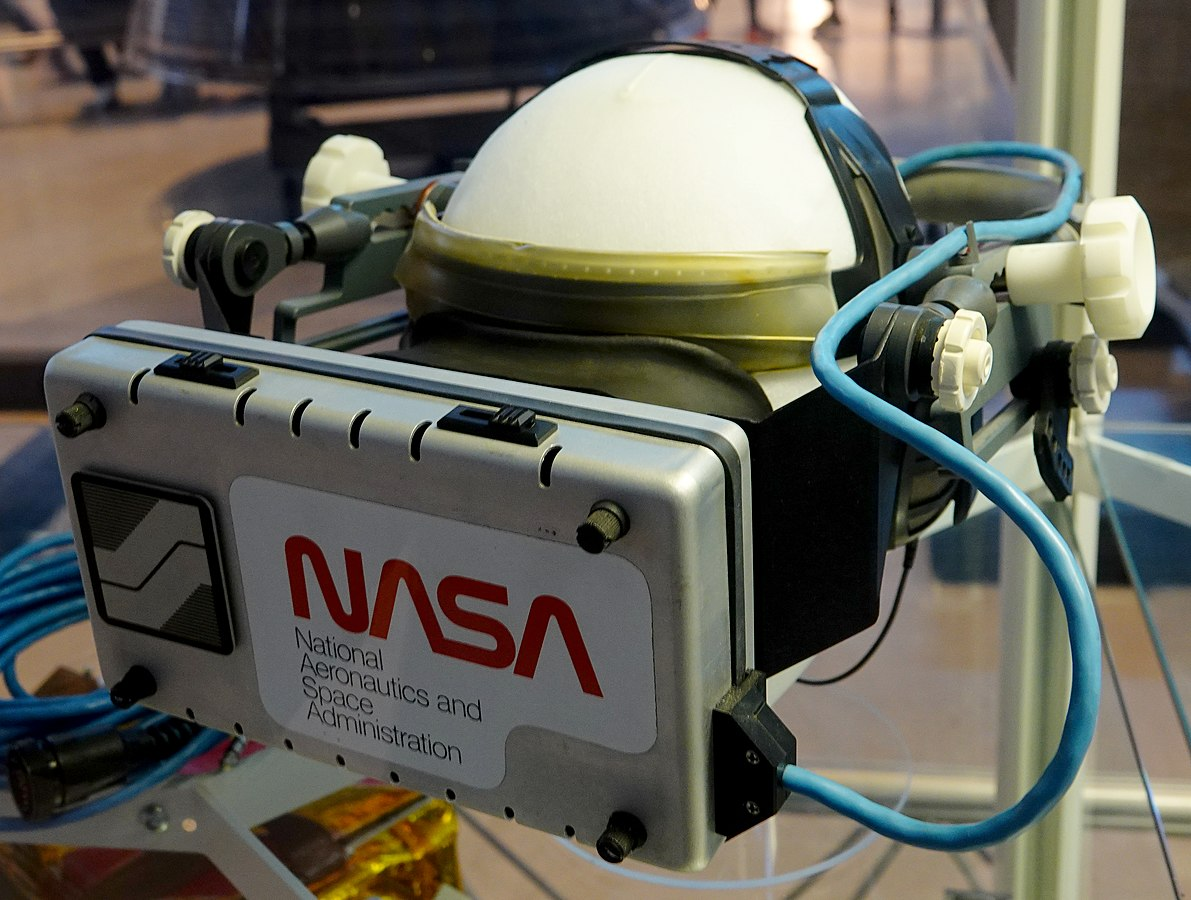
\includegraphics[width=0.75\linewidth]{1191px-Virtual_Reality_Headset_Prototype}
\centering
\caption{This is an example of a figure~\citep{wiki1}}.
\end{figure}
\chapter{Paper 2 - Awesome Paper}
This is your second paper chapter. 
\chapter{Paper 3 - Awesome Paper}
This is your third paper chapter. 
\chapter{Conclusion}
This chapter contains your awesome conlusions.

%----------------------------------------------------------------------------------------
%	BIBLIOGRAPHY
%----------------------------------------------------------------------------------------

\addcontentsline{toc}{chapter}{Bibliography}
\bibliographystyle{plainnat-reversed}  %resource: https://tex.stackexchange.com/questions/375413/how-to-make-last-names-of-authors-appear-first-in-my-bibliography
% do not delete the plainnat-reversed.bst file

\bibliography{bibliography-all}


%----------------------------------------------------------------------------------------

\end{document}  
